% !TeX program = xelatex
\documentclass[12pt, a4paper]{article}
\usepackage{amsmath}
\usepackage{xeCJK}
\usepackage{amsmath}
\usepackage{amssymb}
\usepackage{xcolor}
\usepackage{parskip}
\usepackage{tikz}

\setmainfont{Latin Modern Roman}
\setCJKmainfont{Noto Serif CJK TC}

\title{Ch1. to CH.4 High Light}

\begin{document}
\section*{Signal}
\subsection*{Signal Energy and Power}
\textbf{Continuous time}
\begin{align*}
	E_x &= \lim_{T \to \infty} \int_{-T}^{T} \mid x(t) \mid^2 dt = \int_{-\infty}^{\infty} \mid x(t) \mid^2 dt \quad \in(0, \infty) \\
	P_x &= \lim_{T \to \infty} \frac{1}{2T} \int_{-T}^{T} \mid x(t) \mid^2 dt \quad \in (0, \infty)
\end{align*}

\textbf{Discrete time}
\begin{align*}
	E_x &= \sum_{n=-\infty}^{\infty} \mid x[n] \mid^2 \quad \in (0, \infty) \\
	P_x &= \lim_{N \to \infty} \frac{1}{2N+1} \sum_{n = -N}^{N} \mid x[n] \mid^2 \quad \in(0, \infty)
\end{align*}

\subsection*{Periodic}
利用作圖看是不是週期訊號 \\
\textbf{當訊號為 Discrete time時}滿足週期比較嚴格,一定要在點上面,\color{red}並非\color{black}所有的$\cos$都是週期訊號,一定要符合$\omega_0N = 2\pi m$

\subsection*{Even and Odd Signals}
\begin{align*}
	\varepsilon_v \{ x(t) \} &= \frac {1}{2} [x(t) + x(-t)] \\
	O_v \{ x(t) \} &= \frac {1}{2} [x(t) - x(-t)] \\
\end{align*}
\newpage

\section*{Unit impulse and unit step functions}
\subsection*{Unit impulse}
\textbf{Continous time} \\
Unit impulse 在連續 $t=0$ 的時是 $\infty$,但積分後是1 $\to$ $\int \delta(t) \text{d}t = 1$
$$
\delta(t) = 
\begin{cases}
0, & t \ne 0 \\
\infty, & t = 0
\end{cases}
$$

\textbf{Discrete time} \\
Unit impulse 在離散 $n=0$ 的時候是1,其他時候是0
$$
\delta[n] = 
\begin{cases}
0, & n \ne 0 \\
1, & n = 0
\end{cases}
$$
\subsection*{Unit step function}
$$
u[n] = 
\begin{cases}
0, & n < 0 \\
1, & n \ge 0
\end{cases}
$$
$$
u(t) = 
\begin{cases}
0, & t < 0 \\
1, & t \ge 0
\end{cases}
$$
\subsection*{Proof $\int \delta(t) \text{d}t =1$}
$$
\delta(t) = 
\begin{cases}
\frac{1}{\Delta}, & 0 \le t \le \Delta \\
0
\end{cases}
$$
$$
\int_{0}^{\Delta} \delta_{\Delta}(t) \text{d}t = 1
$$
Therefore
$$
\delta(t) = \lim_{\Delta \to0}
\begin {cases}
\infty, & t = 0 \\
0, & t \ne 0
\end {cases}
$$
$$
\int_{0^-}^{0^+} \delta(t) \text{d}t = 1
$$
\newpage

\section*{System Properties}
\subsection*{Memoryless}
Input 的時序必須和 Output 的時序\textbf{完全一模一樣},不能有過去及未來。
$$
y(t) = [x(t) + x(t)^2]^2
$$
\subsection*{Invertibility}
這比較難一點,需要找出 Inverse system。或是可以從找出兩個不同的 Input 但是有相同的 Output 的反例來判斷。
\subsection*{Causulity}
Output 只和過去的 Input 有關。看他的時間只要沒跟未來有關就是 Causlity。
\subsection*{Stability}
使用 BIBO(Bounded Input Bounded Output) 來判斷,若 Input 為有限值, Output 也是有限值,則這個系統 Stable。\\
\textit{Example:}
\begin{align*}
	&y[n] = x[n-1] \\
	&\left| x[n] \right| < B \to \left|y[n] \right| = \left| x[n-1] \right| < B < \infty
\end{align*}
\subsection*{Linear}
線性系統的特性是 superposition,所以可以使用 $x_1 \to y1$, $x_2 \to y2$ 然後令 $x_3 = \alpha x_1 + \beta x_2$ 看 $y_3$ 是否等於 $\alpha y_1 + \beta y_2$,若成立,則此系統為 linear。
\subsection*{Time-Invarient}
非時變系統是相同的 Input 不會隨著輸入時間的不同,而有不同的 Output。利用將 Input 向右平移 $t_0$(延遲 $t_0$)看 Output 是否也向右平移 $t_0$(延遲 $t_0$)來判斷是否為 time-invarient。
\newpage

\section*{LTI(Linear Time-Invariant) Systems}
LTI system 是先將 $\delta$ 函數丟入 system 產生對應的響應 $h$ 然後將 input 和 h 做 convolution 就可以得到 input 丟入系統所對應的output
\begin{center}
\tikzset{every picture/.style={line width=0.75pt}} %set default line width to 0.75pt        

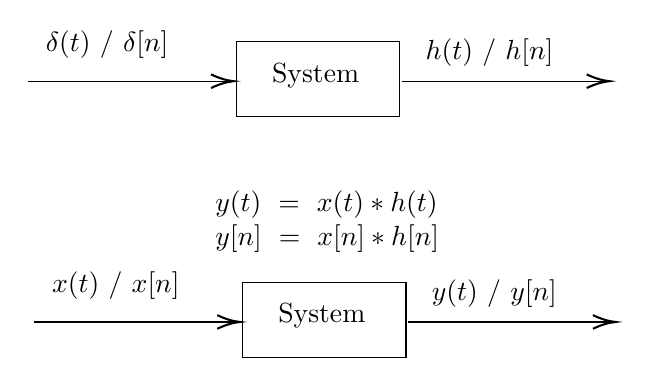
\begin{tikzpicture}[x=0.75pt,y=0.75pt,yscale=-1,xscale=1]
%uncomment if require: \path (0,300); %set diagram left start at 0, and has height of 300

%Shape: Rectangle [id:dp4204380002688358] 
\draw   (297,99.92) -- (375.77,99.92) -- (375.77,135.92) -- (297,135.92) -- cycle ;
%Straight Lines [id:da23613823984617388] 
\draw    (196.77,118.92) -- (293.77,118.92) ;
\draw [shift={(295.77,118.92)}, rotate = 180] [color={rgb, 255:red, 0; green, 0; blue, 0 }  ][line width=0.75]    (10.93,-3.29) .. controls (6.95,-1.4) and (3.31,-0.3) .. (0,0) .. controls (3.31,0.3) and (6.95,1.4) .. (10.93,3.29)   ;
%Straight Lines [id:da6308882612547787] 
\draw    (376.77,118.92) -- (474.77,118.92) ;
\draw [shift={(476.77,118.92)}, rotate = 180] [color={rgb, 255:red, 0; green, 0; blue, 0 }  ][line width=0.75]    (10.93,-3.29) .. controls (6.95,-1.4) and (3.31,-0.3) .. (0,0) .. controls (3.31,0.3) and (6.95,1.4) .. (10.93,3.29)   ;
%Shape: Rectangle [id:dp5949065708697123] 
\draw   (300,215.92) -- (378.77,215.92) -- (378.77,251.92) -- (300,251.92) -- cycle ;
%Straight Lines [id:da4813794065172372] 
\draw    (199.77,234.92) -- (296.77,234.92) ;
\draw [shift={(298.77,234.92)}, rotate = 180] [color={rgb, 255:red, 0; green, 0; blue, 0 }  ][line width=0.75]    (10.93,-3.29) .. controls (6.95,-1.4) and (3.31,-0.3) .. (0,0) .. controls (3.31,0.3) and (6.95,1.4) .. (10.93,3.29)   ;
%Straight Lines [id:da1899703445501454] 
\draw    (379.77,234.92) -- (477.77,234.92) ;
\draw [shift={(479.77,234.92)}, rotate = 180] [color={rgb, 255:red, 0; green, 0; blue, 0 }  ][line width=0.75]    (10.93,-3.29) .. controls (6.95,-1.4) and (3.31,-0.3) .. (0,0) .. controls (3.31,0.3) and (6.95,1.4) .. (10.93,3.29)   ;

% Text Node
\draw (313,109) node [anchor=north west][inner sep=0.75pt]   [align=left] {System};
% Text Node
\draw (204,93.4) node [anchor=north west][inner sep=0.75pt]    {$\delta ( t) \ /\ \delta [ n]$};
% Text Node
\draw (387,97.4) node [anchor=north west][inner sep=0.75pt]    {$h( t) \ /\ h[ n]$};
% Text Node
\draw (316,225) node [anchor=north west][inner sep=0.75pt]   [align=left] {System};
% Text Node
\draw (207,209.4) node [anchor=north west][inner sep=0.75pt]    {$x( t) \ /\ x[ n]$};
% Text Node
\draw (390,213.4) node [anchor=north west][inner sep=0.75pt]    {$y( t) \ /\ y[ n]$};
% Text Node
\draw (279,169.4) node [anchor=north west][inner sep=0.75pt]    {$ \begin{array}{l}
y( t) \ =\ x( t) *h( t)\\
y[ n] \ =\ x[ n] *h[ n]
\end{array}$};
\end{tikzpicture}
\end{center}
\subsection*{Convolution}
\textbf{Continous time}
$$
y(t) = x(t)*h(t) = \int_{-\infty}^{\infty} x(\tau)h(t-\tau)\text{d}\tau
$$
\textbf{Discrete time}
$$
y[n] = x[n]*h[n] = \sum_{k=-\infty}^{\infty} x[k]h[n-k]
$$
\subsection*{Important equivlent}
\textbf{Discrete time}
\begin{align*}
	x[n] &= x[n]*\delta[n] \\
	x[n+k] &= x[n]*\delta[n+k] \\
\end{align*}
\textbf{Continous time}
\begin{align*}
	x(t) &= x(t)*\delta(t) \\
	x(t+k) &= x(t)*\delta(t+k)
\end{align*}


\subsection*{Properties of convoluation}
\subsubsection*{Commutative}
\textbf{Discrete time} $x[n]*h[n] = h[n]*x[n]$
$$
\sum_{k=-\infty}^{\infty} x[k]h[n-k] = \sum_{k=-\infty}^{\infty} h[k]x[n-k]
$$
\textbf{Continous time} $x(t)*h(t) = h(t)*x(t)$
$$
\int_{-\infty}^{\infty} x(\tau)h(t-\tau)\text{d}\tau = \int_{-\infty}^{\infty} h(\tau)x(t-\tau)\text{d}\tau
$$

\subsubsection*{Distributive}
\textbf{Discrete time} $x[n]*(h_1[n] + h_2[n]) = x[n]*h_1[n] + x[n]*h_2[n]$ \\
\textbf{Continous time} $x(t)*(h_1(t) + h_2(t)) = x(t)*h_1(t) + x(t)*h_2(t)$

\subsubsection*{Additive(Linear)}
\textbf{Discrete time} $(x_1[n]+x_2[n])*h[n] = x_1[n]*h[n] + x_2[n]*h[n]$ \\
\textbf{Continous time} $(x_1(t)+x_2(t))*h(t) = x_1(t)*h(t) + x_2(t)*h(t)$

\subsubsection*{Associative}
\textbf{Discrete time} $x[n]*(h_1[n]*h_2[n]) = (x[n]*h_1[n])*h_2[n]$ \\
\textbf{Continous time} $x(t)*(h_1(t)*h_2(t)) = (x(t)*h_1(t))*h_2(t)$
\begin{center}


\tikzset{every picture/.style={line width=0.75pt}} %set default line width to 0.75pt        

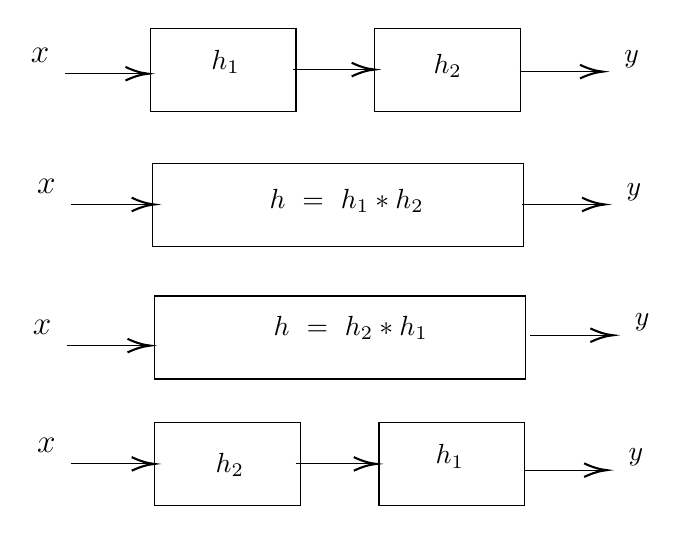
\begin{tikzpicture}[x=0.75pt,y=0.75pt,yscale=-1,xscale=1]
%uncomment if require: \path (0,300); %set diagram left start at 0, and has height of 300

%Shape: Rectangle [id:dp8805200523913231] 
\draw   (259,32) -- (329,32) -- (329,72) -- (259,72) -- cycle ;
%Shape: Rectangle [id:dp8235779632151183] 
\draw   (367,32) -- (437,32) -- (437,72) -- (367,72) -- cycle ;
%Shape: Rectangle [id:dp6359840555839769] 
\draw   (259.77,97) -- (438.77,97) -- (438.77,137) -- (259.77,137) -- cycle ;
%Shape: Rectangle [id:dp08006179479990161] 
\draw   (260.77,161) -- (439.77,161) -- (439.77,201) -- (260.77,201) -- cycle ;
%Shape: Rectangle [id:dp7700226635379218] 
\draw   (261,222) -- (331,222) -- (331,262) -- (261,262) -- cycle ;
%Shape: Rectangle [id:dp28557116730178933] 
\draw   (369,222) -- (439,222) -- (439,262) -- (369,262) -- cycle ;
%Straight Lines [id:da5761705109627222] 
\draw    (217.77,53.92) -- (255.77,53.92) ;
\draw [shift={(257.77,53.92)}, rotate = 180] [color={rgb, 255:red, 0; green, 0; blue, 0 }  ][line width=0.75]    (10.93,-3.29) .. controls (6.95,-1.4) and (3.31,-0.3) .. (0,0) .. controls (3.31,0.3) and (6.95,1.4) .. (10.93,3.29)   ;
%Straight Lines [id:da23176508793808637] 
\draw    (220.77,116.92) -- (258.77,116.92) ;
\draw [shift={(260.77,116.92)}, rotate = 180] [color={rgb, 255:red, 0; green, 0; blue, 0 }  ][line width=0.75]    (10.93,-3.29) .. controls (6.95,-1.4) and (3.31,-0.3) .. (0,0) .. controls (3.31,0.3) and (6.95,1.4) .. (10.93,3.29)   ;
%Straight Lines [id:da324493480437135] 
\draw    (218.77,184.92) -- (256.77,184.92) ;
\draw [shift={(258.77,184.92)}, rotate = 180] [color={rgb, 255:red, 0; green, 0; blue, 0 }  ][line width=0.75]    (10.93,-3.29) .. controls (6.95,-1.4) and (3.31,-0.3) .. (0,0) .. controls (3.31,0.3) and (6.95,1.4) .. (10.93,3.29)   ;
%Straight Lines [id:da6440074473499616] 
\draw    (220.77,241.92) -- (258.77,241.92) ;
\draw [shift={(260.77,241.92)}, rotate = 180] [color={rgb, 255:red, 0; green, 0; blue, 0 }  ][line width=0.75]    (10.93,-3.29) .. controls (6.95,-1.4) and (3.31,-0.3) .. (0,0) .. controls (3.31,0.3) and (6.95,1.4) .. (10.93,3.29)   ;
%Straight Lines [id:da11729276240151787] 
\draw    (327.77,51.92) -- (364.77,51.92) ;
\draw [shift={(366.77,51.92)}, rotate = 180] [color={rgb, 255:red, 0; green, 0; blue, 0 }  ][line width=0.75]    (10.93,-3.29) .. controls (6.95,-1.4) and (3.31,-0.3) .. (0,0) .. controls (3.31,0.3) and (6.95,1.4) .. (10.93,3.29)   ;
%Straight Lines [id:da5575163341209703] 
\draw    (328.77,241.92) -- (365.77,241.92) ;
\draw [shift={(367.77,241.92)}, rotate = 180] [color={rgb, 255:red, 0; green, 0; blue, 0 }  ][line width=0.75]    (10.93,-3.29) .. controls (6.95,-1.4) and (3.31,-0.3) .. (0,0) .. controls (3.31,0.3) and (6.95,1.4) .. (10.93,3.29)   ;
%Straight Lines [id:da22189195806400008] 
\draw    (436.77,52.92) -- (474.77,52.92) ;
\draw [shift={(476.77,52.92)}, rotate = 180] [color={rgb, 255:red, 0; green, 0; blue, 0 }  ][line width=0.75]    (10.93,-3.29) .. controls (6.95,-1.4) and (3.31,-0.3) .. (0,0) .. controls (3.31,0.3) and (6.95,1.4) .. (10.93,3.29)   ;
%Straight Lines [id:da9013427813386689] 
\draw    (437.77,116.92) -- (475.77,116.92) ;
\draw [shift={(477.77,116.92)}, rotate = 180] [color={rgb, 255:red, 0; green, 0; blue, 0 }  ][line width=0.75]    (10.93,-3.29) .. controls (6.95,-1.4) and (3.31,-0.3) .. (0,0) .. controls (3.31,0.3) and (6.95,1.4) .. (10.93,3.29)   ;
%Straight Lines [id:da40073295423463773] 
\draw    (441.77,179.92) -- (479.77,179.92) ;
\draw [shift={(481.77,179.92)}, rotate = 180] [color={rgb, 255:red, 0; green, 0; blue, 0 }  ][line width=0.75]    (10.93,-3.29) .. controls (6.95,-1.4) and (3.31,-0.3) .. (0,0) .. controls (3.31,0.3) and (6.95,1.4) .. (10.93,3.29)   ;
%Straight Lines [id:da6729366003239877] 
\draw    (438.77,244.92) -- (476.77,244.92) ;
\draw [shift={(478.77,244.92)}, rotate = 180] [color={rgb, 255:red, 0; green, 0; blue, 0 }  ][line width=0.75]    (10.93,-3.29) .. controls (6.95,-1.4) and (3.31,-0.3) .. (0,0) .. controls (3.31,0.3) and (6.95,1.4) .. (10.93,3.29)   ;

% Text Node
\draw (200,40.4) node [anchor=north west][inner sep=0.75pt]  [font=\large]  {$x$};
% Text Node
\draw (203,103.4) node [anchor=north west][inner sep=0.75pt]  [font=\large]  {$x$};
% Text Node
\draw (201,171.4) node [anchor=north west][inner sep=0.75pt]  [font=\large]  {$x$};
% Text Node
\draw (203,228.4) node [anchor=north west][inner sep=0.75pt]  [font=\large]  {$x$};
% Text Node
\draw (486,41.4) node [anchor=north west][inner sep=0.75pt]    {$y$};
% Text Node
\draw (487,105.4) node [anchor=north west][inner sep=0.75pt]    {$y$};
% Text Node
\draw (491,168.4) node [anchor=north west][inner sep=0.75pt]    {$y$};
% Text Node
\draw (488,233.4) node [anchor=north west][inner sep=0.75pt]    {$y$};
% Text Node
\draw (287,41.4) node [anchor=north west][inner sep=0.75pt]    {$h_{1}$};
% Text Node
\draw (394,43.4) node [anchor=north west][inner sep=0.75pt]    {$h_{2}$};
% Text Node
\draw (289,235.4) node [anchor=north west][inner sep=0.75pt]    {$h_{2}$};
% Text Node
\draw (395,231.4) node [anchor=north west][inner sep=0.75pt]    {$h_{1}$};
% Text Node
\draw (317,169.4) node [anchor=north west][inner sep=0.75pt]    {$h\ =\ h_{2} *h_{1}$};
% Text Node
\draw (315,108.4) node [anchor=north west][inner sep=0.75pt]    {$h\ =\ h_{1} *h_{2}$};
\end{tikzpicture}
\end{center}
\newpage

\subsection*{Properties of LTI system}
\subsubsection*{Memoryless / with Memory}
LTI system 只有在 $h[n] = k\delta[n]$ 或是 $h(t) = k\delta(t)$是\color{red} Memoryless \color{black},其他時候都是 \color{blue} with Memory \color{black}

\subsubsection*{Causality}
Causal 只會發生在$h[n] = 0$, for $n<0$ 或是 $h(t) = 0$, for $t<0$
\begin{align*}
	y[n] &= \sum_{k = -\infty}^{\infty} x[k]h[n-k] \\
			 &= \sum_{k = -\infty}^{\infty} h[k]x[n-k] \\
			 &= h[0]x[n] + h[1]x[n-1] + h[2]x[n-2] + ... &&\qquad \color{green} x[n-k] \color{black} \\
			 &+ h[-1]x[n+1] + h[-2]x[n+2] + h[-3]x[n+3] &&\qquad \color{red} x[n+k] \text{未來訊號} \color{black} \\
	y(t) &= \int_{-\infty}^{\infty} x(\tau)h(t-\tau)\text{d}\tau \\
			 &= \int_{-\infty}^{\infty} h(\tau)x(t-\tau)\text{d}\tau \\
			 &= \int_{-\infty}^{0} h(\tau) \color{red}\underbrace {\color{black}x(t-\tau)}_{\text{未來部分}}\color{black}\text{d}\tau + \int_{0}^{\infty} h(\tau) \color{green}\underbrace{\color{black}x(t-\tau)}_{\text{過去部分}}\color{black} \text{d}\tau
\end{align*}

\subsubsection*{Invertibility}
如果系統的 impulse response($h(t)$, $h[n]$) 是 invertible 則它有 LTI inverse impulse response ($h_I(t)$, $h_I[n]$) \\
\begin{align*}
	h(t)*h_I(t) &= \delta(t) \\
	h[n]*h_I[n] &= \delta[n]
\end{align*}
\begin{center}


\tikzset{every picture/.style={line width=0.75pt}} %set default line width to 0.75pt        

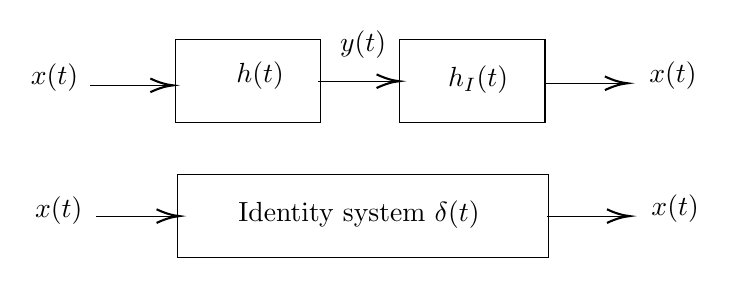
\begin{tikzpicture}[x=0.75pt,y=0.75pt,yscale=-1,xscale=1]
%uncomment if require: \path (0,300); %set diagram left start at 0, and has height of 300

%Shape: Rectangle [id:dp8805200523913231] 
\draw   (253,85) -- (323,85) -- (323,125) -- (253,125) -- cycle ;
%Shape: Rectangle [id:dp8235779632151183] 
\draw   (361,85) -- (431,85) -- (431,125) -- (361,125) -- cycle ;
%Shape: Rectangle [id:dp6359840555839769] 
\draw   (253.77,150) -- (432.77,150) -- (432.77,190) -- (253.77,190) -- cycle ;
%Straight Lines [id:da5761705109627222] 
\draw    (211.77,106.92) -- (249.77,106.92) ;
\draw [shift={(251.77,106.92)}, rotate = 180] [color={rgb, 255:red, 0; green, 0; blue, 0 }  ][line width=0.75]    (10.93,-3.29) .. controls (6.95,-1.4) and (3.31,-0.3) .. (0,0) .. controls (3.31,0.3) and (6.95,1.4) .. (10.93,3.29)   ;
%Straight Lines [id:da23176508793808637] 
\draw    (214.77,169.92) -- (252.77,169.92) ;
\draw [shift={(254.77,169.92)}, rotate = 180] [color={rgb, 255:red, 0; green, 0; blue, 0 }  ][line width=0.75]    (10.93,-3.29) .. controls (6.95,-1.4) and (3.31,-0.3) .. (0,0) .. controls (3.31,0.3) and (6.95,1.4) .. (10.93,3.29)   ;
%Straight Lines [id:da11729276240151787] 
\draw    (321.77,104.92) -- (358.77,104.92) ;
\draw [shift={(360.77,104.92)}, rotate = 180] [color={rgb, 255:red, 0; green, 0; blue, 0 }  ][line width=0.75]    (10.93,-3.29) .. controls (6.95,-1.4) and (3.31,-0.3) .. (0,0) .. controls (3.31,0.3) and (6.95,1.4) .. (10.93,3.29)   ;
%Straight Lines [id:da22189195806400008] 
\draw    (430.77,105.92) -- (468.77,105.92) ;
\draw [shift={(470.77,105.92)}, rotate = 180] [color={rgb, 255:red, 0; green, 0; blue, 0 }  ][line width=0.75]    (10.93,-3.29) .. controls (6.95,-1.4) and (3.31,-0.3) .. (0,0) .. controls (3.31,0.3) and (6.95,1.4) .. (10.93,3.29)   ;
%Straight Lines [id:da9013427813386689] 
\draw    (431.77,169.92) -- (469.77,169.92) ;
\draw [shift={(471.77,169.92)}, rotate = 180] [color={rgb, 255:red, 0; green, 0; blue, 0 }  ][line width=0.75]    (10.93,-3.29) .. controls (6.95,-1.4) and (3.31,-0.3) .. (0,0) .. controls (3.31,0.3) and (6.95,1.4) .. (10.93,3.29)   ;

% Text Node
\draw (182,95.4) node [anchor=north west][inner sep=0.75pt]  [font=\normalsize]  {$x( t)$};
% Text Node
\draw (184,159.4) node [anchor=north west][inner sep=0.75pt]  [font=\normalsize]  {$x( t)$};
% Text Node
\draw (480,94.4) node [anchor=north west][inner sep=0.75pt]    {$x( t)$};
% Text Node
\draw (481,158.4) node [anchor=north west][inner sep=0.75pt]    {$x( t)$};
% Text Node
\draw (281,94.4) node [anchor=north west][inner sep=0.75pt]    {$h( t)$};
% Text Node
\draw (383,96.4) node [anchor=north west][inner sep=0.75pt]    {$h_{I}( t)$};
% Text Node
\draw (282,161.4) node [anchor=north west][inner sep=0.75pt]    {$\text{Identity system } \delta ( t)$};
% Text Node
\draw (331,79.4) node [anchor=north west][inner sep=0.75pt]    {$y( t)$};
\end{tikzpicture}
\end{center}
\newpage

\subsubsection*{Stability}
\textbf{Discrete time:} given bounded input $\left|x[n]\right|<B$, for all $n$ \\
magnitude of the output is
\begin{align*}
	\left|y[n]\right| &= \left|\sum_{k=-\infty}^{\infty}h[k]x[n-k]\right| \\
										&\leq \sum_{k=-\infty}^{\infty}\left|h[k]\right| \cdot \left|x[n-k]\right| \\
										&\leq B \sum_{k=-\infty}^{\infty} \left|h[k]\right|
\end{align*}
The impulse response is absolutely summable that
$$
\sum_{k=-\infty}^{\infty} \left|h[k]\right|<\infty
$$
\\ \\
\textbf{Continous time:} given bounded input $\left|x(t)\right|<B$, for all $t$ \\
magnitude of the output is
\begin{align*}
	\left|y(t)\right| &= \left|\int_{-\infty}^{\infty}h(\tau)x(t-\tau)\text{d}\tau\right|\\
										&\leq \int_{-\infty}^{\infty}\left|h(\tau)\right|\cdot\left|x(t-\tau)\right| \text{d}\tau \\
										&\leq B\int_{-\infty}^{\infty}\left|h(\tau)\right|\text{d}\tau
\end{align*}
The impulse response is absolutely summable that
$$
\int_{-\infty}^{\infty} \left|h(\tau)\right|<\infty
$$
\newpage

\subsection*{Singularity Functions}
\subsubsection*{Differentiator}
Unit impulse response of a diffrentiator
$$
h(t) = \frac{\text{d}\delta(t)}{\text{d}t} \equiv u_1'(t)
$$
Convolution will be 
$$
\frac{\text{d}x(t)}{\text{d}t}= x(t)*u_1'(t)
$$
\textbf{\textit{pf.}}
\begin{align*}
	\frac{\text{d}x(t)}{\text{d}t} &= \lim_{\Delta t \to 0} \frac{x(t)-x(t-\Delta t)}{\Delta t} \\
																 &= \lim_{\Delta t \to 0} \frac{x(t)*(\color{red}\delta(t)-\delta(t-\Delta t)\color{black})}{\Delta t} \\
																 &= x(t) * \color{red} \frac{\delta(t)}{\text{d}t} \color{black}
\end{align*}

\subsubsection*{Integrator}
Unit impulse response of a diffrentiator
$$
h(t) = \int_{-\infty}^{t}\delta(\tau)\text{d}\tau \equiv u(t)
$$
Convolution will be 
$$
x(t)*u(t) = \int_{-\infty}^{\infty}x(\tau)u(t-\tau)\text{d}\tau = \int_{-\infty}^{t}x(t)\text{d}\tau
$$
\newpage

\section*{Fourier Series Representation}
\subsection*{Continous time}
\begin{align*}
	x(t) &= \sum_{k=-\infty}^{\infty}a_ke^{jk\omega_0t}\\
	a_k &= \frac{1}{T} \int_T x(t) \cdot e^{-jk\omega_0t} \text{d}t
\end{align*}
$a_k$ 就是將 $x(t)$ 對基底$e^{jk\omega_0t}$ 用內積得到投影的長度,因為複數內積要取 conjugate 所以會有負號,連續的 $\omega_0 = 2\pi / T$
\subsubsection*{Properties}

\begin{center}
	\begin{tabular} { |c|c c| }
		\hline
		Property & Periodic Signal & Fourier Series Coefficients \\
		\hline
		Linearty & $Ax(t) + By(t)$ & $Aa_k + Bb_k$ \\
		Time Shifting & $t-t_0$ & $a_ke^{-jk\omega_0t_0}$ \\
		Frequency Shifting & $e^{jM\omega_0t}x(t)$ & $a_{k-M}$ \\
		Conjugation & $x^*(t)$ & $a^*_{-k}$ \\
		Multiplication & $x(t)y(t)$ & $\sum_{l=-\infty}^{\infty}a_l b_{k-l}$ \\
		Differentiation & $\frac{\text{d}x(t)}{\text{d}t}$ & $jk\omega_0a_k$ \\
		Integration & $\int_{-\infty}^{t}x(t)\text{d}t$ & $\left(\frac{1}{jk\omega_0}\right)a_k$ \\
		\hline
	\end{tabular}
\end{center}
Conjugate symmetry for real signals($x(t)$ is real)
\begin{align*}
	\begin{cases}
		a_k = a^*_{-k} \\
		\Re \{a_k\} = \Re \{a_{-k}\} \\
		\Im  \{a_k\} = -\Im \{a_{-k}\} \\
		\left|a_k\right| = \left|a_{-k}\right| \\
		\angle a_k = -\angle a_k
	\end{cases}
\end{align*}

\begin{minipage}[t]{0.3 \textwidth}
\begin{align*}
	\begin{cases}
	  x_e(t) = Ev \{x(t)\} \\
		x_o(t) = Od \{x(t)\}
	\end{cases}
\end{align*}
\end{minipage}
\hfill
\begin{minipage}[t]{0.3 \textwidth}
\begin{align*}
	\begin{cases}
		\Re \{a_k\} \\
	  j\Im \{a_k\}	\\
\end{cases}
\end{align*}
\end{minipage}
\\ \\
Parseval's Relation
$$
\frac{1}{T} \int_T \left|x(t)\right|^2 \text{d}t = \sum_{k=-\infty}^{\infty} \left|a_k\right|^2
$$
\newpage

\subsection*{Discrete time}
\begin{align*}
	x[n] &= \sum_{k=\langle N \rangle}a_ke^{jk\omega_0n}\\
	a_k &= \frac{1}{N} \sum_{n=\langle N \rangle} x[n] \cdot e^{-jk\omega_0n}
\end{align*}
$a_k$ 就是將 $x[n]$ 對基底$e^{jk\omega_0n}$ 用內積得到投影的長度,因為複數內積要取 conjugate 所以會有負號,離散的 $\omega_0 = 2\pi / N$
\subsubsection*{Properties}

\begin{center}
	\begin{tabular} { |c|c c| }
		\hline
		Property & Periodic Signal & Fourier Series Coefficients \\
		\hline
		Linearty & $Ax[n] + By[n]$ & $Aa_k + Bb_k$ \\
		Time Shifting & $n-n_0$ & $a_ke^{-jk\omega_0n_0}$ \\
		Frequency Shifting & $e^{jM\omega_0t}x[n]$ & $a_{k-M}$ \\
		Conjugation & $x^*[n]$ & $a^*_{-k}$ \\
		Multiplication & $x[n]y[n]$ & $\sum_{l=-\infty}^{\infty}a_l b_{k-l}$ \\
		First Difference & $x[n] - x[n-1]$ & $(1-e^{-jk\omega_0})a_k$ \\
		Running Sum & $\sum_{k = -\infty}^{n} x[k]$ & $\left(\frac{1}{1-e^{-jk\omega_0}}\right)a_k$ \\
		\hline
	\end{tabular}
\end{center}
Conjugate symmetry for real signals($x(t)$ is real)
\begin{align*}
	\begin{cases}
		a_k = a^*_{-k} \\
		\Re \{a_k\} = \Re \{a_{-k}\} \\
		\Im  \{a_k\} = -\Im \{a_{-k}\} \\
		\left|a_k\right| = \left|a_{-k}\right| \\
		\angle a_k = -\angle a_k
	\end{cases}
\end{align*}

\begin{minipage}[t]{0.3 \textwidth}
\begin{align*}
	\begin{cases}
	  x_e(t) = Ev \{x(t)\} \\
		x_o(t) = Od \{x(t)\}
	\end{cases}
\end{align*}
\end{minipage}
\hfill
\begin{minipage}[t]{0.3 \textwidth}
\begin{align*}
	\begin{cases}
		\Re \{a_k\} \\
	  j\Im \{a_k\}	\\
\end{cases}
\end{align*}
\end{minipage}
\\ \\
Parseval's Relation
$$
\frac{1}{N} \sum_{n = \langle N \rangle} \left|x(t)\right|^2 \text{d}t = \sum_{k=\langle N \rangle} \left|a_k\right|^2
$$
\newpage

\subsection*{With LTI system}
\textbf{Continuous time} \\
Let $H(j\omega)$ as frequency response of the system
$$
H(j\omega) = \int_{-\infty}^{\infty} h(t)e^{-j\omega t}\text{d}t
$$
From Superposition property
$$
x(t) = \sum_{k = -\infty}^{\infty}a_ke^{jk\omega_0t} \longrightarrow y(t) = \sum_{k = -\infty}^{\infty}a_k H(jk\omega_0)e^{jk\omega_0t}
$$

\textbf{Discrete time} \\
Let $H(e^{j\omega})$ as frequency response of the system
$$
H(e^{j\omega}) = \sum_{-\infty}^{\infty} h[n]e^{-j\omega n}
$$
From Superposition property
$$
x[n] = \sum_{k = \langle N \rangle}a_ke^{jk\omega_0n} \longrightarrow y(t) = \sum_{k = \langle N \rangle}a_k H(e^{j\omega}))e^{jk\omega_0n}
$$
\newpage

\section*{Continuous Time Fourier Transform}
\begin{align*}
	X(j\omega) &= \int_{-\infty}^{\infty} x(t)e^{-j\omega t}\text{d}t &&\qquad \color{red} \text {Fourier Transform} \color{black} \\
	x(t) &= \frac{1}{2 \pi} \int_{-\infty}^{\infty}X(j\omega)e^{j\omega t}\text{d}\omega &&\qquad \color{red} \text {Inverse Fourier Transform} \color{black}
\end{align*}

\subsection*{Common fourier transform}
For $\alpha>0$ $e^{-\alpha t}u(t)$
$$
x(t) = e^{-\alpha t}u(t) \xrightarrow{F} \frac{1}{\alpha + j\omega}
$$
\textbf{\textit{Pf.}}
\begin{align*}
	X(j\omega) &= \int_{-\infty}^{\infty} x(t) e^{-j\omega t} \text{d}t
						 = \int_{-\infty}^{\infty} e^{-\alpha t} e^{-j \omega t} \text{d} \\
						 &= \left. \frac{-1}{\alpha + j\omega} e^{-(a+j\omega)t} \right|_0^{\infty} 
						 = \frac{1}{\alpha + j\omega}
\end{align*}
\\
\begin{minipage}[t]{0.5 \textwidth}
	方波的 Fourier transform
	$$
  x(t) = \begin{cases} 1, \quad \left| t \right| \leq T_1 \\
	0, \quad \left| t \right| > T_1 \end{cases}
	$$
\end{minipage}
\hfill
\begin{minipage}[t]{0.3 \textwidth}
\centering
\tikzset{every picture/.style={line width=0.75pt}} %set default line width to 0.75pt     
\begin{tikzpicture}[x=0.75pt,y=0.75pt,yscale=-1,xscale=1, baseline=(current bounding box.north)]
%uncomment if require: \path (0,300); %set diagram left start at 0, and has height of 300

%Shape: Rectangle [id:dp28551682930557276] 
\draw   (319.99,150.4) -- (360.66,150.4) -- (360.66,190.4) -- (319.99,190.4) -- cycle ;
%Shape: Axis 2D [id:dp00630958994675257] 
\draw  (266,190.27) -- (420.99,190.27)(340.38,101) -- (340.38,201) (413.99,185.27) -- (420.99,190.27) -- (413.99,195.27) (335.38,108) -- (340.38,101) -- (345.38,108)  ;

% Text Node
\draw (355.28,198.4) node [anchor=north west][inner sep=0.75pt]  [font=\scriptsize]  {$T_{1}$};
% Text Node
\draw (307.94,196.73) node [anchor=north west][inner sep=0.75pt]  [font=\scriptsize]  {$-T_{1}$};
% Text Node
\draw (332.94,81.4) node [anchor=north west][inner sep=0.75pt]  [font=\scriptsize]  {$x( t)$};
\end{tikzpicture}
\end{minipage}
$$
x(t) \xrightarrow{F} 2\frac{\sin(\omega T_1)}{\omega} = 2T_1 \operatorname{sinc}(\frac{\omega \pi}{\pi})
$$
\textbf{\textit{Pf.}}
\begin{align*}
	X(j\omega) &= \int_{-T_1}^{T_1} 1 \cdot e^{-j\omega t} \text{d}t \\
						 &= \frac{-1}{j\omega}\left( e^{-j\omega T_1} - e^{j\omega T_1} \right) \\
						 &= \frac{2 \sin(\omega T_1)}{\omega} = 2T_1 \frac{\sin(\omega T_1)}{\omega T_1} \\
						 &= 2T_1 \operatorname{sinc}(\frac{\omega \pi}{\pi})
\end{align*}

\end{document}
